\documentclass[onecolumn, letter, 11pt]{article}

\usepackage{fourier}
\usepackage[utf8]{inputenc}
\usepackage[sumlimits]{amsmath}
\usepackage{graphicx}
\usepackage[spanish]{babel}
\usepackage{amsfonts}
\usepackage{amssymb}
\usepackage{amsthm}
\usepackage{geometry}

\geometry{left=2.5cm,right=2.5cm,top=2.5cm,bottom=2.5cm}


\title{Examen rápido No. 8}
\author{Inteligencia Artificial, curso 2017b\\ \textsc{Julio Waissman Vilanova}}
\date{}


\begin{document}

\maketitle

\section{Red Bayesiana}

 De acuerdo a la red bayesiana mostrada en la figura siguiente responde cuales de las siguientes afirmaciones son falsas o verdaderas (2 puntos cada
respuesta):

\begin{center}
   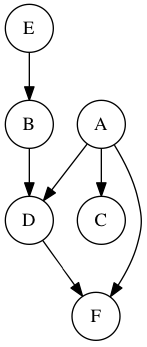
\includegraphics[width=0.2\textwidth]{modelo_red_bayesiana.png}
\end{center}

\begin{enumerate}
\item[\line(1,0){22}] E es independiente de F
\item[\line(1,0){22}] A es independiente de E
\item[\line(1,0){22}] A es independiente de E conociendo B
\item[\line(1,0){22}] A es independiente de E conociendo D
\item[\line(1,0){22}] A es independiente de B
\item[\line(1,0){22}] A es independiente de B conociendo D
\item[\line(1,0){22}] A es independiente de B conociendo F
\item[\line(1,0){22}] C es independiente de D
\item[\line(1,0){22}] C es independiente de D conociendo A
\item[\line(1,0){22}] C es independiente de D conociendo F
\end{enumerate}

Si consideramos que las variables A, B, C, D son binarias, y las variables E y F tienen 3
valores posibles, ¿Cual es el número mínimo de parámetros que se requiere calcular para
calcular las tablas de probabilidad condicional (CPT's) de la red bayesiana? (10 puntos)

\vspace{1cm}

\line(1,0){435}

\section{Inferencia bayesiana}

De acuerdo a la siguiente red bayesiana, realiza lo que se pide

\begin{center}
  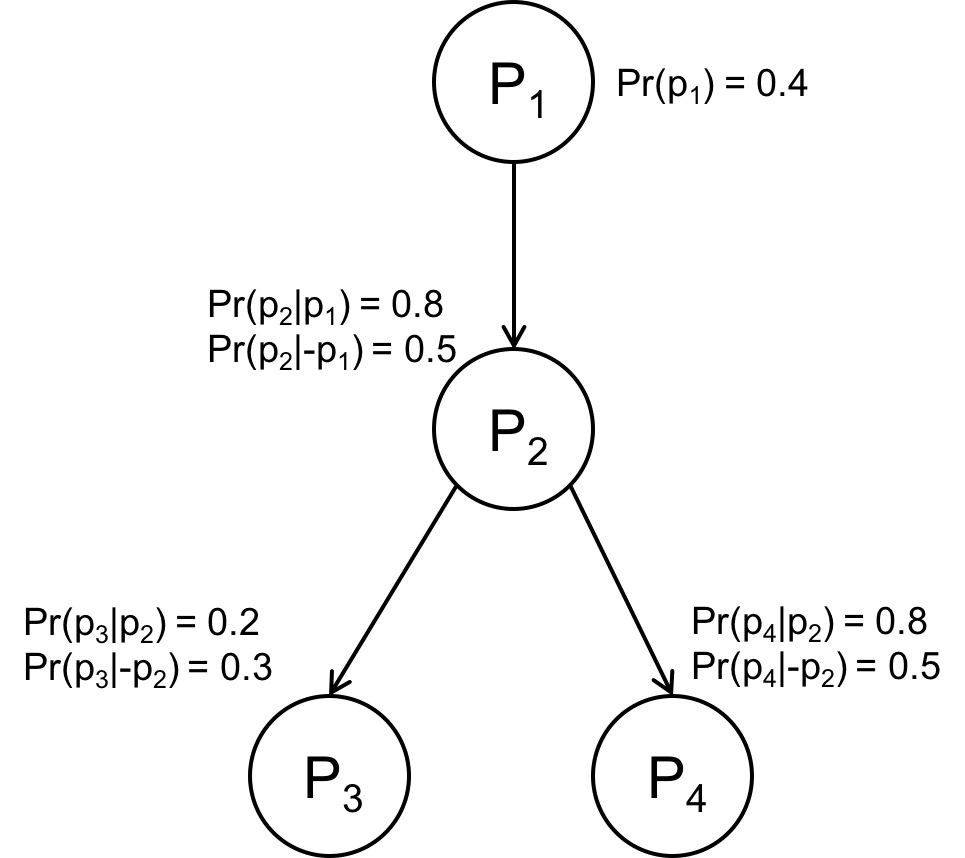
\includegraphics[width=0.6\textwidth]{bayes_leve.png}
\end{center}

\begin{enumerate}
\item Calcula $\Pr(-p_3)$:
\item Calcula $\Pr(p_2|p_3)$:
\item Calcula $\Pr(p_1|p_2, -p_3)$:
\item Calcula $\Pr(p_1|-p_3, p_4)$:
\item Calcula aproximadamente $\Pr(p_1|p_2, -p_3)$ con el métdo de
  muestreo con pesos de verosimilitud. Genera al menos unas 20
  muestras y compara el resultado con lo obtenido por inferencia
  exacta.
\end{enumerate}


\end{document}
